%
% scilabisnotnaive.tex --
%   Some notes about floating point issues in Scilab.
%
% Copyright 2008 Michael Baudin
%
\documentclass[12pt]{article}

%% Good fonts for PDF
\usepackage[cyr]{aeguill}

%% Package for page headers
\usepackage{fancyhdr}

%% Package to include graphics
%% Comment for DVI
\usepackage[pdftex]{graphicx}

%% Figures formats: jpeg or pdf
%% Comment for DVI
\DeclareGraphicsExtensions{.jpg,.pdf}

%% Package to create Hyperdocuments
%% Comment for DVI
\usepackage[pdftex,colorlinks=true,linkcolor=blue,citecolor=blue,urlcolor=blue]{hyperref}

%% Package to control printed area size
\usepackage{anysize}
%% ...by defining margins {left}{right}{top}{bottom}
\marginsize{22mm}{14mm}{12mm}{25mm}

%% Package used to include a bibliography
\usepackage{natbib}

%% R for real numbers
\usepackage{amssymb}

%% User defined commands

%% Figure reference
\newcommand{\figref}[1]{figure~\ref{#1}}

%% Equation reference
\newcommand{\Ref}[1]{(\ref{#1})}

%% Emphasize a word or a group of words
\newcommand{\empha}[1]{\textit{\textbf{#1}}}

%% Derivation operators
\newcommand{\D}{\partial}
\newcommand{\Dt}{\partial_t}
\newcommand{\Dx}{\partial_x}
\newcommand{\Dy}{\partial_y}

\usepackage{url}

% Scilab macros
\newcommand{\scimacro}[1]{\textit{#1}}
\newcommand{\scicommand}[1]{\textit{#1}}

% To highlight source code
\usepackage{listings}
\usepackage{algorithmic}

% Define theorem environments 
\newtheorem{theorem}{Theorem}[section]
\newtheorem{lemma}[theorem]{Lemma}
\newtheorem{proposition}[theorem]{Proposition}
\newtheorem{corollary}[theorem]{Corollary}

\newenvironment{proof}[1][Proof]{\begin{trivlist}
\item[\hskip \labelsep {\bfseries #1}]}{\end{trivlist}}
\newenvironment{definition}[1][Definition]{\begin{trivlist}
\item[\hskip \labelsep {\bfseries #1}]}{\end{trivlist}}
\newenvironment{example}[1][Example]{\begin{trivlist}
\item[\hskip \labelsep {\bfseries #1}]}{\end{trivlist}}
\newenvironment{remark}[1][Remark]{\begin{trivlist}
\item[\hskip \labelsep {\bfseries #1}]}{\end{trivlist}}

\newcommand{\qed}{\nobreak \ifvmode \relax \else
      \ifdim\lastskip<1.5em \hskip-\lastskip
      \hskip1.5em plus0em minus0.5em \fi \nobreak
      \vrule height0.75em width0.5em depth0.25em\fi}

% Maths shortcuts 
\newcommand{\RR}{\mathbb{R}}

% Algorithms
\usepackage{algorithm2e}
%%\usepackage{algorithmic}

\begin{document}
\author{Michael Baudin}
\date{February 2009}
\title{Scilab is not na�ve}
\maketitle
\begin{abstract}
Most of the time, the mathematical formula is 
directly used in the Scilab source code. 
But, in many algorithms, some additionnal work is 
performed, which takes into account the fact that 
the computer do not process mathematical real values,
but performs computations with their floating 
point representation.
The goal of this article is to show that, in many
situations, Scilab is not na�ve and use algorithms
which have been specifically tailored for floating point 
computers. We analyse in this article the 
particular case of the quadratic equation, the 
complex division and the numerical derivatives, 
and show that one these examples, the na�ve algorithm 
is not sufficiently accurate. 
\end{abstract}

\tableofcontents

\chapter{Introduction}

In this introductory chapter, we make an overview of simplex-based algorithms.
We present the main features of the \scifunction{neldermead} component, and 
show how to use the component with a simple example.

\section{Overview}

The Nelder-Mead simplex algorithm \cite{citeulike:3009487}, published in 1965, is an enormously 
popular search method for multidimensional unconstrained optimization. 
The Nelder-Mead algorithm should not be confused with the (probably) 
more famous simplex algorithm of Dantzig for linear programming. The 
Nelder-Mead algorithm is especially popular in the fields of chemistry, 
chemical engineering, and medicine. Two measures of the ubiquity of the 
Nelder-Mead algorithm are that it appears in the best-selling handbook 
Numerical Recipes and in Matlab. In \cite{Torczon89multi-directionalsearch},
Virginia Torczon writes: "Margaret Wright has stated that over
fifty percent of the calls received by the support group for the NAG
software library concerned the version of the Nelder-Mead 
simplex algorithm to be found in that library". No derivative of the cost function is 
required, which makes the algorithm interesting for noisy problems.

The Nelder-Mead algorithm falls in the more general class of direct 
search algorithms. These methods use values of $f$ taken from a set of 
sample points and use that information to continue the sampling. The 
Nelder-Mead algorithm maintains a simplex which are approximations of an 
optimal point. The vertices are sorted according to the objective 
function values. The algorithm attemps to replace the worst vertex with 
a new point, which depends on the worst point and the centre of the best 
vertices. 

The goal of this toolbox is to provide a Nelder-Mead (1965) direct search optimization method to solve the 
following unconstrained optimization problem
\begin{eqnarray}
\min f(\bx)
\end{eqnarray}
where $\bx\in \RR^n$, $n$ is the number of optimization parameters and $f$ is the objective 
function $f:\RR^n\rightarrow \RR$.
In order to solve the unconstrained optimization problem, the Nelder-Mead 
algorithm uses a variable shape simplex. The toolbox also provide Spendley's et al. 
algorithm \cite{Spendley1962} (1962), which uses a fixed shape simplex. Historically, the algorithm created  
by Nelder and Mead was designed as an improvement on Spendley's et al. algorithm.
The Box complex algorithm \cite{Box1965} (1965), which is an extension of Spendley's  et al. algorithm, solves the 
following constrained problem
\begin{eqnarray}
&&\min f(\bx)\\
&&\ell_i \leq x_i \leq u_i, \qquad i = 1,n\\
&&g_j(\bx)\geq 0, \qquad j = 1, m\\
\end{eqnarray}
where $m$ is the number of nonlinear, positive constraints and $\ell_i,u_i\in \RR^n$ are the lower 
and upper bounds of the variables.

The Nelder-Mead algorithm may be used in the following optimization context :
\begin{itemize}
\item there is no need to provide the derivatives of the objective function,
\item the number of parameters is small (up to 10-20),
\item there are bounds and/or non linear constraints.
\end{itemize}

The internal design of the system is based on the following components.
\begin{itemize}
\item The "neldermead" component provides various simplex-based 
algorithms and manages for Nelder-Mead specific settings, such as the 
method to compute the initial simplex and the specific termination 
criteria.
\item The "fminsearch" component provides a Scilab commands which aims 
at behaving as Matlab's fminsearch. Specific terminations criteria, 
initial simplex and auxiliary settings are automatically configured so 
that the behavior of Matlab's fminsearch is exactly reproduced.
\item The "optimset" and "optimget" components provide Scilab commands 
to emulate their Matlab counterparts.
\item The "nmplot" component provides features to 
produce directly output pictures for Nelder-Mead algorithm.
\end{itemize}
The current toolbox is based on (and therefore requires) the following components.
\begin{itemize}
\item The "optimbase" component provides an abstract class for a general optimization 
component, including the number of variables, the minimum and maximum 
bounds, the number of non linear inequality constraints, the logging 
system, various termination criteria, the cost function, etc...
\item The "optimsimplex" component provides a class to manage a simplex made of an 
arbitrary number of vertices, including the computation of a simplex by 
various methods (axes, regular, Pfeffer's, randomized bounds), the 
computation of the size by various methods (diameter, sigma +, sigma-, 
etc...) and many algorithms to perform reflections and shrinkages.
\end{itemize}

The following is a list of features the Nelder-Mead algorithm currently provides :
\begin{itemize}
\item manage various simplex initializations
  \begin{itemize}
  \item initial simplex given by user,
  \item initial simplex computed with a length and along the coordinate axes,
  \item initial regular simplex computed with Spendley et al. formula
  \item initial simplex computed by a small perturbation around the initial guess point
  \end{itemize}
\item manage cost function
  \begin{itemize}
  \item optionnal additionnal argument
  \item direct communication of the task to perform : cost function or inequality constraints
  \end{itemize}
\item manage various termination criteria 
  \begin{itemize}
  \item maximum number of iterations, 
  \item tolerance on function value (relative or absolute),
  \item tolerance on x (relative or absolute),
  \item tolerance on standard deviation of function value (original termination criteria in [3]),
  \item maximum number of evaluations of cost function,
  \item absolute or relative simplex size,
  \end{itemize}
\item manage the history of the convergence, including :
  \begin{itemize}
  \item the history of function values,
  \item the history of optimum point,
  \item the history of simplices,
  \item the history of termination criterias,
  \end{itemize}
\item provide a plot command which allows to graphically see the history of the simplices toward the optimum,
\item provide query functions for 
  \begin{itemize}
  \item the status of the optimization process,
  \item the number of iterations, 
  \item the number of function evaluations, 
  \item the status of execution, 
  \item the function value at initial point, 
  \item the function value at optimal point, 
  \item etc...
  \end{itemize}
\item Spendley et al. fixed shaped algorithm,
\item Kelley restart based on simplex gradient,
\item O'Neill restart based on factorial search around optimum,
\item Box-like method managing bounds and nonlinear inequality constraints based on arbitrary number of vertices in the simplex.
\end{itemize}

\section{How to use the Toolbox}

The design of the toolbox is based on the creation of 
a new token by the \scifunction{neldermead\_new} function.
The Nelder-Mead object associated with this token can then 
be configured with \scifunction{neldermead\_configure} and queried 
with \scifunction{neldermead\_cget}. For example, the
\scifunction{neldermead\_configure} command allows to configure the 
number of variables, the objective function and the initial guess.

The main command of the toolbox is the \scifunction{neldermead\_search} command, which
solves the optimization problem. After an optimization has been performed,
the \scifunction{neldermead\_get} command allows to retrieve the optimum $x^\star$,
as well as other parameters, such as the number of iterations performed, the number 
of evaluations of the function, etc...

Once the optimization is finished, the \scifunction{neldermead\_destroy} function 
deletes the object.

\section{An example}

In the following example, we search the minimum of the 2D Rosenbrock function \cite{citeulike:1903787}, 
defined by
\begin{eqnarray}
f(x_1,x_2) = 100(x_2 - x_1)^2 + (1-x_1)^2
\end{eqnarray}

The following Scilab script allows to find the solution of the problem. 
We begin by defining the function \scifunction{rosenbrock} which computes the Rosenbrock function. 
The traditionnal initial guess $(-1.2 , 1.0)$ is used, which corresponds 
to the "-x0" key. The initial simplex is computed along 
the axes with a length equal to 0.1. We want to use the Nelder-Mead algorithm with variable simplex size 
is used, which corresponds to the "variable" value of the "-method" option. 
The verbose mode is enabled so that messages are generated during the algorithm. 
After the optimization is performed, the optimum is retrieved with quiery features.

\lstset{language=scilabscript}
\begin{lstlisting}
function y = rosenbrock (x)
  y = 100*(x(2)-x(1)^2)^2 + (1-x(1))^2;
endfunction
nm = neldermead_new ();
nm = neldermead_configure(nm,"-numberofvariables",2);
nm = neldermead_configure(nm,"-x0",[-1.2 1.0]');
nm = neldermead_configure(nm,"-simplex0method","axes");
nm = neldermead_configure(nm,"-simplex0length",0.1);
nm = neldermead_configure(nm,"-method","variable");
nm = neldermead_configure(nm,"-verbose",1);
nm = neldermead_configure(nm,"-function",rosenbrock);
nm = neldermead_search(nm);
xopt = neldermead_get(nm,"-xopt")
fopt = neldermead_get(nm,"-fopt")
status = neldermead_get(nm,"-status")
nm = neldermead_destroy(nm);
\end{lstlisting}

This produces the following output.

\lstset{language=scilabscript}
\begin{lstlisting}
-->nm = neldermead_search(nm);
Function Evaluation #1 is [24.2] at [-1.2 1]
Function Evaluation #1 is [24.2] at [-1.2 1]
Function Evaluation #2 is [8.82] at [-1.1 1]
Function Evaluation #3 is [16.4] at [-1.2 1.1]
Step #1 : order
=================================================================
Iteration #1 (total = 1)
Function Eval #3
Xopt : -1.1 1
Fopt : 8.820000e+000
DeltaFv : 1.538000e+001
Center : -1.1666667 1.0333333
Size : 1.414214e-001
Vertex #1/3 : fv=8.820000e+000, x=-1.100000e+000 1.000000e+000
Vertex #2/3 : fv=1.640000e+001, x=-1.200000e+000 1.100000e+000
Vertex #3/3 : fv=2.420000e+001, x=-1.200000e+000 1.000000e+000
Reflect
xbar=-1.15 1.05
Function Evaluation #4 is [5.62] at [-1.1 1.1]
xr=[-1.1 1.1], f(xr)=5.620000
Expand
Function Evaluation #5 is [4.428125] at [-1.05 1.15]
xe=-1.05 1.15, f(xe)=4.428125
  > Perform Expansion
Sort
[...]
=================================================================
Iteration #56 (total = 56)
Function Eval #98
Xopt : 0.6537880 0.4402918
Fopt : 1.363828e-001
DeltaFv : 1.309875e-002
Center : 0.6788120 0.4503999
Size : 6.945988e-002
Vertex #1/3 : fv=1.363828e-001, x=6.537880e-001 4.402918e-001
Vertex #2/3 : fv=1.474625e-001, x=7.107987e-001 4.799712e-001
Vertex #3/3 : fv=1.494816e-001, x=6.718493e-001 4.309367e-001
Reflect
xbar=0.6822933 0.4601315
Function Evaluation #99 is [0.1033237] at [0.6927374 0.4893262]
xr=[0.6927374 0.4893262], f(xr)=0.103324
Expand
Function Evaluation #100 is [0.1459740] at [0.7031815 0.5185210]
xe=0.7031815 0.5185210, f(xe)=0.145974
  > Perform reflection
Sort
=================================================================
Iteration #57 (total = 57)
Function Eval #100
Xopt : 0.6927374 0.4893262
Fopt : 1.033237e-001
DeltaFv : 4.413878e-002
Center : 0.6857747 0.4698631
Size : 6.262139e-002
Vertex #1/3 : fv=1.033237e-001, x=6.927374e-001 4.893262e-001
Vertex #2/3 : fv=1.363828e-001, x=6.537880e-001 4.402918e-001
Vertex #3/3 : fv=1.474625e-001, x=7.107987e-001 4.799712e-001
Terminate with status : maxfuneval
-->xopt = neldermead_get(nm,"-xopt")
 xopt  =
 
    0.6927374  
    0.4893262  
 
-->fopt = neldermead_get(nm,"-fopt")
 fopt  =
 
    0.1033237  
 
-->status = neldermead_get(nm,"-status")
 status  =
 
 maxfuneval   
\end{lstlisting}

\section{Help, demonstrations and unit tests}

For a complete presentation of the functions and options, the reader 
should consult the help which is provided with the component.
The main menu of the help associated with the optimization 
module is presented in figures \ref{fig-intro-help} and \ref{fig-intro-helpfminsearch}.
The corresponding pages provide a complete documentation for the 
corresponding functions, as well as many sample uses.

\begin{figure}
\begin{center}
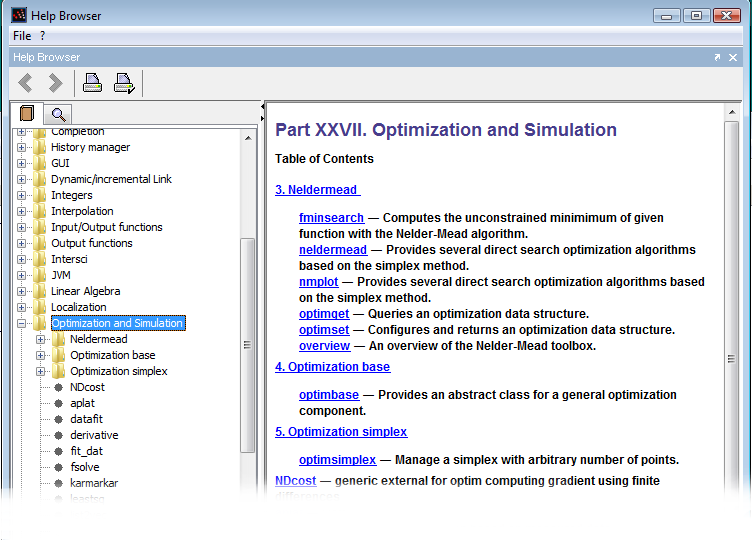
\includegraphics[width=15cm]{introduction-help.png}
\end{center}
\caption{Built-in help for the Nelder-Mead component}
\label{fig-intro-help}
\end{figure}

\begin{figure}
\begin{center}
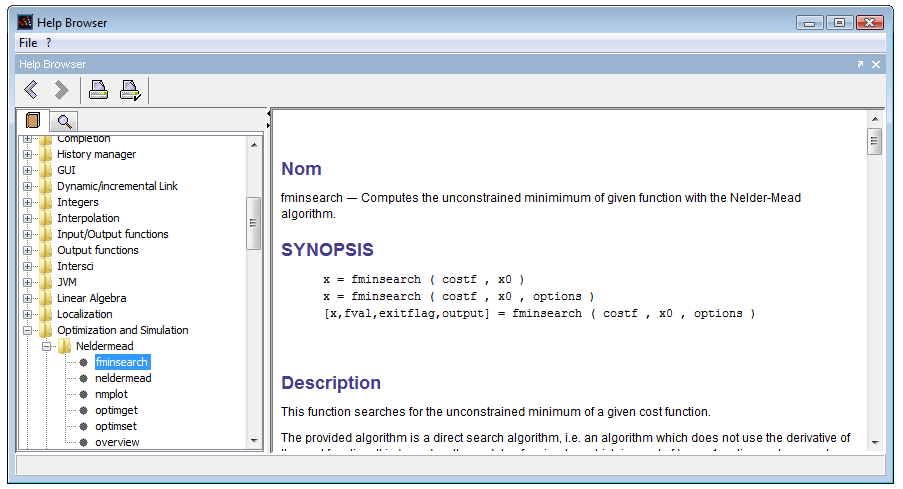
\includegraphics[width=15cm]{introduction-help-fminsearch.png}
\end{center}
\caption{Built-in help for the \scifunction{fminsearch} function}
\label{fig-intro-helpfminsearch}
\end{figure}

Several demonstrations are provided with the component. These 
are available from the "Demonstration" menu of the Scilab console
and are presented in figure \ref{fig-intro-demos}.

\begin{figure}
\begin{center}
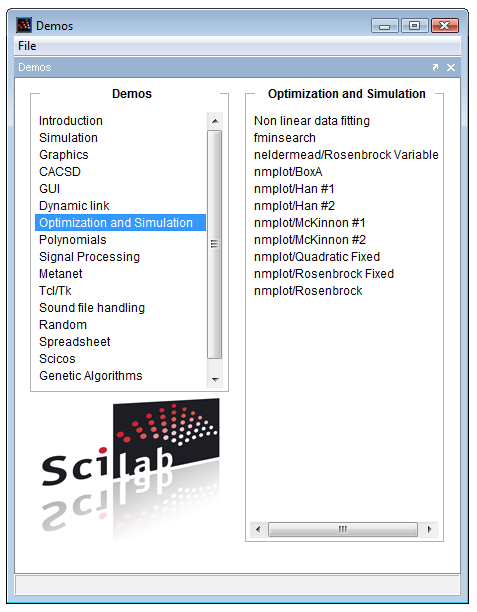
\includegraphics[width=10cm]{introduction-demos.png}
\end{center}
\caption{Built-in demonstration scripts for the Nelder-Mead component}
\label{fig-intro-demos}
\end{figure}

The following script shows where the demonstration scripts are 
available from the Scilab installation directory.

\lstset{language=scilabscript}
\begin{lstlisting}
-->cd SCI/modules/optimization/demos/neldermead
 ans  =
 
 D:\Programs\SCFD8E~1\modules\optimization\demos\neldermead   
 
-->ls *.sce
 ans  =
 
!nmplot_rosenbrock.sce        !
!                             !
!nmplot_rosenbrock.fixed.sce  !
!                             !
!nmplot_quadratic.fixed.sce   !
!                             !
!nmplot_mckinnon2.sce         !
!                             !
!nmplot_mckinnon.sce          !
!                             !
!nmplot_han2.sce              !
!                             !
!nmplot_han1.sce              !
!                             !
!nmplot_boxproblemA.sce       !
!                             !
!neldermead_rosenbrock.sce    !
!                             !
!neldermead.dem.sce           !
!                             !
!fminsearch.sce               !
\end{lstlisting}

These components were developped based on unit tests, which are 
provided with Scilab.
These unit tests are located in the "SCI/modules/optimization/tests/unit\_tests"
directory, under the "neldermead", "optimsimplex" and "optimbase" directories.
Each unit test correspond to a .tst file. These tests are covering most 
(if not all) the features provided by the components. This is why there are 
a good source of information on how to use the functions.






% Scilab ( http://www.scilab.org/ ) - This file is part of Scilab
% Copyright (C) 2008-2010 - Digiteo - Michael Baudin
%
% This file must be used under the terms of the CeCILL.
% This source file is licensed as described in the file COPYING, which
% you should have received as part of this distribution.  The terms
% are also available at
% http://www.cecill.info/licences/Licence_CeCILL_V2-en.txt

\section{Quadratic equation}

In this section, we analyze the computation of the roots of a quadratic polynomial.
As we shall see, there is a whole \emph{world} from the mathematical formulas to the 
implementation of such computations. In the first part, we briefly report the formulas which allow to 
compute the real roots of a quadratic equation with real coefficients.
We then present the naive algorithm based on these mathematical formulas. 
In the second part, we make some experiments in Scilab and compare our
naive algorithm with the \scifun{roots} Scilab function.
In the third part, we analyze why and how floating point numbers must be 
taken into account when the roots of a quadratic are required.

\subsection{Theory}

In this section, we present the mathematical formulas which allow to compute the 
real roots of a quadratic polynomial with real coefficients.
We chose to begin by the example of a quadratic equation, because most of 
us exactly know (or \emph{think} we know) how to solve such an equation with a computer.

Assume that $a, b, c \in \RR$ are given coefficients and $a\neq 0$. 
Consider the following quadratic \cite{wikipediaquadratic,wikipedialossofsign,mathworldquadratic} equation:
\begin{eqnarray}
\label{eq-quadratic}
a x^2 + b x + c = 0,
\end{eqnarray}
where $x\in\RR$ is the unknown.

Let us define by $\Delta=b^2-4ac$ the discriminant of the quadratic equation.
We consider the mathematical solution of the quadratic equation, 
depending on the sign of the discriminant $\Delta=b^2 - 4ac$.
\begin{itemize}
\item If $\Delta> 0$, there are two real roots: 
% Keep two equations for the root selection explanation
\begin{eqnarray}
x_- &=& \frac{-b- \sqrt{\Delta}}{2a}, \label{real:x-} \\
x_+ &=& \frac{-b+ \sqrt{\Delta}}{2a}. \label{real:x+}
\end{eqnarray}
\item If $\Delta=0$, there is one double root:
\begin{eqnarray}
\label{realdouble:x-+}
x_\pm &=& -\frac{b}{2a}.
\end{eqnarray}
\item If $\Delta< 0$, there are two complex roots:
\begin{eqnarray}
\label{complex:x-+}
x_\pm &=&\frac{-b}{2a} \pm i \frac{\sqrt{-\Delta}}{2a}.
\end{eqnarray}
\end{itemize}

We now consider a simplified algorithm where we only compute the real roots of the 
quadratic, assuming that $\Delta>0$.
This naive algorithm is presented in figure \ref{naive-quadratic}.

\begin{algorithm}[htbp]
\SetKwInOut{Input}{input}\SetKwInOut{Output}{output}
\Input{$a,b,c$}
\Output{$x_-$, $x_+$}
$\Delta:= b^2-4ac$\;
$s:= \sqrt{\Delta}$\;
$x_-:= (-b-s)/(2a)$\;
$x_+:= (-b+s)/(2a)$\;
\caption{Naive algorithm to compute the real roots of a quadratic equation. - We assume that $\Delta> 0$.}
\label{naive-quadratic}
\end{algorithm}

%%%%%%%%%%%%%%%%%%%%%%%%%%%%%%%%%%%%%%%%%%%%%%%%%%%%%%%%%%%%%%%%%
\subsection{Experiments}

In this section, we compare our naive algorithm with the \scifun{roots} function.
We begin by defining a function which naively implements the mathematical formulas.
Then we use our naive function on two particular examples. 
In the first example, we focus on massive cancellation and in the second example, we 
focus on overflow problems.

The following Scilab function \scifun{myroots} is a straightforward implementation
of the previous formulas. It takes as input the coefficients of the quadratic, stored in the 
vector variable \scivar{p}, and returns the two roots in the vector \scivar{r}.
\lstset{language=scilabscript}
\begin{lstlisting}
function r=myroots(p)
  c=coeff(p,0);
  b=coeff(p,1);
  a=coeff(p,2);
  r(1)=(-b+sqrt(b^2-4*a*c))/(2*a);
  r(2)=(-b-sqrt(b^2-4*a*c))/(2*a);
endfunction
\end{lstlisting}

%%%%%%%%%%%%%%%%%%%%%%%%%%%%%%%%%%%%%%%%%%%%%%%%%%%%%%%%%%%%%%%%%
\subsubsection{Massive cancellation}
\label{section-exp-quadraticrounding}

\index{cancellation}
\index{massive cancellation}
We analyze the rounding errors which are 
appearing when the discriminant of the quadratic equation 
is such that $b^2\gg 4ac$.
We consider the following quadratic equation 
\begin{eqnarray}
\label{sinn-eq-roundingerror}
\epsilon x^2 + (1/\epsilon)x - \epsilon = 0
\end{eqnarray}
with $\epsilon>0$. For example, consider the special case $\epsilon=0.0001=10^{-4}$. 
The discriminant of this equation is $\Delta = 1/\epsilon^2+4\epsilon^2$.

The two real solutions of the quadratic equation are
\begin{eqnarray}
\label{sinn-eq-roundingerror-roots}
x_- = \frac{-1/\epsilon- \sqrt{1/\epsilon^2+4\epsilon^2}}{2\epsilon}, \qquad
x_+ = \frac{-1/\epsilon+ \sqrt{1/\epsilon^2+4\epsilon^2}}{2\epsilon}.
\end{eqnarray}
These roots are approximated by 
\begin{eqnarray}
\label{sinn-eq-roundingerror-roots-approx}
x_- \approx  -1/\epsilon^2, \qquad
x_+ \approx  \epsilon^2,
\end{eqnarray}
when $\epsilon$ is close to zero.
We now consider the limit of the two roots when $\epsilon \rightarrow 0$. We have 
\begin{eqnarray}
\lim_{\epsilon\rightarrow 0} x_- = -\infty, \qquad
\lim_{\epsilon\rightarrow 0} x_+ = 0.
\end{eqnarray}

\index{\scifun{roots}}
In the following Scilab script, we compare the roots computed by the \scifun{roots}
function and the roots computed by our naive function. We begin by creating 
a polynomial with the \scifun{poly} function, which is given the coefficients of 
the polynomial. Only the positive root $x_+ \approx \epsilon^2$ is considered in this 
test. Indeed, the $x_-$ root is so that $x_- \rightarrow -\infty$ in both 
implementations.
\lstset{language=scilabscript}
\begin{lstlisting}
p=poly([-0.0001 10000.0 0.0001],"x","coeff");
e1 = 1e-8;
roots1 = myroots(p);
r1 = roots1(1);
roots2 = roots(p);
r2 = roots2(1);
error1 = abs(r1-e1)/e1;
error2 = abs(r2-e1)/e1;
printf("Expected : %e\n", e1);
printf("Naive method : %e (error=%e)\n", r1,error1);
printf("Scilab method : %e (error=%e)\n", r2, error2);
\end{lstlisting}

The previous script produces the following output.
\lstset{language=scilabscript}
\begin{lstlisting}
Expected : 1.000000e-008
Naive method : 9.094947e-009 (error=9.050530e-002)
Scilab method : 1.000000e-008 (error=1.654361e-016)
\end{lstlisting}

We see that the naive method produces a root which has no significant digit 
and a relative error which is 14 orders of magnitude greater than the relative 
error of the Scilab root.

This behavior is explained by the fact that the expression for the 
positive root $x_+$ given by the equality \ref{real:x+} is numerically evaluated 
as following. We first consider how the discriminant $\Delta = 1/\epsilon^2+4\epsilon^2$ 
is computed. The term $1/\epsilon^2$ is equal to 100000000 and the term $4\epsilon^2$ 
is equal to 0.00000004. Therefore, the sum of these two terms is equal to 100000000.000000045.
Hence, the square root of the discriminant is 
\begin{eqnarray}
\sqrt{1/\epsilon^2+4\epsilon^2} = 10000.000000000001818989.
\end{eqnarray}
As we see, the first digits are correct, but the last digits 
are subject to rounding errors. When the expression $-1/\epsilon+ \sqrt{1/\epsilon^2+4\epsilon^2}$
is evaluated, the following computations are performed~:
\begin{eqnarray}
-1/\epsilon+ \sqrt{1/\epsilon^2+4\epsilon^2} &=& -10000.0 + 10000.000000000001818989 \\
  &=& 0.0000000000018189894035
\end{eqnarray}
We see that the result is mainly driven by the cancellation of significant digits.

We may think that the result is extreme, but it 
is not. For example, consider the case where we reduce further the value of $\epsilon$ down to 
$\epsilon=10^{-11}$, we get the following output :
\begin{lstlisting}
Expected : 1.000000e-022
Naive method : 0.000000e+000 (error=1.000000e+000)
Scilab method : 1.000000e-022 (error=1.175494e-016)
\end{lstlisting}

The relative error is this time 16 orders of magnitude 
greater than the relative error of the Scilab root.
There is no significant decimal digit in the result. 
In fact, the naive implementation computes a false root $x_+$ even for 
a value of epsilon equal to $\epsilon=10^{-3}$, where the relative 
error is 7 orders of magnitude greater than the relative error produced by the 
\scifun{roots} function.

%%%%%%%%%%%%%%%%%%%%%%%%%%%%%%%%%%%%%%%%%%%%%%%%%%%%%%%%%%%%%%%%%
\subsubsection{Overflow}
\label{section-exp-quadraticoverflow}

\index{overflow}
In this section, we analyse the overflow which appears  
when the discriminant of the quadratic equation 
is such that $b^2- 4ac$ is not representable as a double.
We consider the following quadratic equation 
\begin{eqnarray}
\label{sinn-eq-overflowerror}
x^2 + (1/\epsilon)x + 1 = 0
\end{eqnarray}
with $\epsilon>0$. We especially consider the case $\epsilon\rightarrow 0$. 
The discriminant of this equation is $\Delta=1/\epsilon^2 -4$. Assume that the discriminant is positive.
Therefore, the roots of the quadratic equation are 
\begin{eqnarray}
x_- = \frac{-1/\epsilon- \sqrt{1/\epsilon^2-4}}{2}, \qquad
x_+ = \frac{-1/\epsilon+ \sqrt{1/\epsilon^2-4}}{2}.
\end{eqnarray}
These roots are approximated by 
\begin{eqnarray}
\label{sinn-eq-rootsoverflowapprox}
x_- \approx  -1/\epsilon, \qquad
x_+ \approx  -\epsilon,
\end{eqnarray}
when $\epsilon$ is close to zero.
We now consider the limit of the two roots when $\epsilon \rightarrow 0$. We have 
\begin{eqnarray}
\lim_{\epsilon\rightarrow 0} x_- = -\infty, \qquad
\lim_{\epsilon\rightarrow 0} x_+ = 0^-.
\end{eqnarray}
To create a difficult case, we search $\epsilon$ so that 
$1/\epsilon^2 > 10^{308}$, because we know that $10^{308}$
is the maximum representable double precision floating 
point number. Therefore, we expect that something should go wrong 
in the computation of the expression $\sqrt{1/\epsilon^2-4}$. 
We choose $\epsilon=10^{-155}$.

In the following script, we compare the roots computed by the \scifun{roots}
function and our naive implementation.
\lstset{language=scilabscript}
\begin{lstlisting}
e=1.e-155
a = 1;
b = 1/e;
c = 1;
p=poly([c b a],"x","coeff");
expected = [-e;-1/e];
roots1 = myroots(p);
roots2 = roots(p);
error1 = abs(roots1-expected)/norm(expected);
error2 = abs(roots2-expected)/norm(expected);
printf("Expected : %e %e\n", expected(1),expected(2));
printf("Naive method : %e %e (error=%e %e)\n", ...
  roots1(1),roots1(2), error1(1),error1(2));
printf("Scilab method : %e %e (error=%e %e)\n", ...
  roots2(1),roots2(2), error2(1),error2(2));
\end{lstlisting}

The previous script produces the following output.
\begin{lstlisting}
Expected : -1.000000e-155 -1.000000e+155
Naive method : Inf Inf (error=Nan Nan)
Scilab method : -1.000000e-155 -1.000000e+155 
            (error=0.000000e+000 0.000000e+000)
\end{lstlisting}

In this case, the discriminant $\Delta = b^2-4ac$ has been evaluated as $1/\epsilon^2-4$,
which is approximately equal to $10^{310}$. This number cannot 
be represented in a double precision floating point number. It therefore produces the 
IEEE Infinite number, which is displayed by Scilab as \scivar{Inf}.
The Infinite number is associated with an algebra and functions can perfectly 
take this number as input. Therefore, when the square root function 
must compute $\sqrt{\Delta}$, it produces again \scivar{Inf}. This number is 
then propagated into the final roots.

%%%%%%%%%%%%%%%%%%%%%%%%%%%%%%%%%%%%%%%%%%%%%%%%%%%%%%%%%%%%%%%%%
\subsection{Explanations}

In this section, we suggest robust methods to compute the roots of a 
quadratic equation. 

\index{Jenkins, M. A.}
\index{Traub, J. F.}
The methods presented in this section are extracted from the 
\emph{quad} routine of the \emph{RPOLY} algorithm by
Jenkins and Traub \cite{JenkinsTraub1970,Jenkins1975}. This algorithm is used by Scilab in the 
\scifun{roots} function, where a special case is used when the 
degree of the equation is equal to 2, i.e. a quadratic equation.

%%%%%%%%%%%%%%%%%%%%%%%%%%%%%%%%%%%%%%%%%%%%%%%%%%%%%%%%%%%%%%%%%
\subsubsection{Properties of the roots}

In this section, we present elementary results, which will be 
used in the derivation of robust floating point formulas of the roots 
of the quadratic equation. 

Let us assume that the quadratic equation \ref{eq-quadratic}, with 
real coefficients $a,b,c\in\RR$ and $a>0$ has a positive 
discriminant $\Delta=b^2-4ac$. Therefore, the two real roots of 
the quadratic equation are given by the equations \ref{real:x-} and \ref{real:x+}.
We can prove that the sum and the product of the roots satisfy the equations 
\begin{eqnarray}
\label{eq-rootsprops}
x_- + x_+ =\frac{-b}{a},\qquad
x_- x_+ =\frac{c}{a}.
\end{eqnarray}
Therefore, the roots are the solution of the normalized 
quadratic equation 
\begin{eqnarray}
\label{eq-rootsprops2}
x^2 - (x_- + x_+) x  + x_- x_+ &=&0.
\end{eqnarray}

Another transformation leads to an alternative form of the roots. 
Indeed, the original quadratic equation can be written as a quadratic 
equation of the unknown $1/x$. Consider the quadratic equation \ref{eq-quadratic}
and divide it by $1/x^2$, assuming that $x\neq 0$. This leads to the equation 
\begin{eqnarray}
\label{eq-quadraticinverse}
c(1/x)^2 + b (1/x)  + a &=&0,
\end{eqnarray}
where we assume that $x\neq 0$.
The two real roots of the quadratic equation \ref{eq-quadraticinverse} are 
\begin{eqnarray}
% Keep two equations for the root selection explanation
x_- &=& \frac{2c}{-b+ \sqrt{b^2-4ac}}, \label{real:x-inverse}\\
x_+ &=& \frac{2c}{-b- \sqrt{b^2-4ac}} \label{real:x+inverse}.
\end{eqnarray}
The expressions \ref{real:x-inverse} and \ref{real:x+inverse} can 
also be derived directly from the equations \ref{real:x-} and \ref{real:x+}.
For that purpose, it suffices to multiply their numerator and denominator 
by $-b+ \sqrt{b^2-4ac}$.

%%%%%%%%%%%%%%%%%%%%%%%%%%%%%%%%%%%%%%%%%%%%%%%%%%%%%%%%%%%%%%%%%
\subsubsection{Floating-Point implementation : overview}

The numerical experiments presented in sections \ref{section-exp-quadraticrounding} and
\ref{section-exp-quadraticoverflow} suggest that the floating point implementation
must deal with two different problems:
\begin{itemize}
\item massive cancellation when $b^2\gg 4ac$ because of the cancellation of the 
terms $-b$ and $\pm\sqrt{b^2-4ac}$ which may have opposite signs,
\item overflow in the computation of the square root of the 
discriminant $\sqrt{\pm(b^2-4ac)}$ when $b^2-4ac$ is not representable as 
a floating point number.
\end{itemize}

The cancellation problem occurs only when the discriminant is positive, i.e. only
when there are two real roots. Indeed, the cancellation will not appear when $\Delta<0$,
since the complex roots do not use the sum $-b\pm\sqrt{b^2-4ac}$.
When $\Delta=0$, the double real root does not cause any trouble.
Therefore, we must take into account for the cancellation problem only in the 
equations \ref{real:x-} and \ref{real:x+}.

On the other hand, the overflow problem occurs whatever the sign of the discriminant
but does not occur when $\Delta=0$. Therefore, we must take into account 
for this problem in the equations \ref{real:x-}, \ref{real:x+} and \ref{complex:x-+}.
In section \ref{section-quadratic-fixcancellation}, we focus on the cancellation error while 
the overflow problem is addressed in section \ref{section-quadratic-fixoverflow}.

%%%%%%%%%%%%%%%%%%%%%%%%%%%%%%%%%%%%%%%%%%%%%%%%%%%%%%%%%%%%%%%%%
\subsubsection{Floating-Point implementation : fixing massive cancellation}
\label{section-quadratic-fixcancellation}
In this section, we present the computation of the roots of a 
quadratic equation with protection against massive cancellation. 

When the discriminant $\Delta$ is positive, the massive cancellation problem can be split in two cases:
\begin{itemize}
\item if $b<0$, then $-b-\sqrt{b^2-4ac}$ may suffer of massive cancellation
because $-b$ is positive and $-\sqrt{b^2-4ac}$ is negative,
\item if $b>0$, then $-b+\sqrt{b^2-4ac}$ may suffer of massive cancellation because 
$-b$ is negative and $\sqrt{b^2-4ac}$ is positive.
\end{itemize}
Therefore, 
\begin{itemize}
\item if $b>0$, we should use the expression $-b-\sqrt{b^2-4ac}$,
\item if $b<0$, we should use the expression $-b+\sqrt{b^2-4ac}$.
\end{itemize}
The solution consists in a combination of the following expressions of the 
roots given by, on one hand the equations \ref{real:x-} and \ref{real:x+},
and, on the other hand the equations \ref{real:x-inverse} and \ref{real:x+inverse}.
We pick the formula so that the sign of $b$ is the 
same as the sign of the square root.
The following choice allow to solve the massive cancellation problem:
\begin{itemize}
\item if $b<0$, then compute $x_-$ from \ref{real:x-inverse}, else 
(if $b>0$), compute $x_-$ from \ref{real:x-},
\item if $b<0$, then compute $x_+$ from \ref{real:x+}, else 
(if $b>0$), compute $x_+$ from \ref{real:x+inverse}.
\end{itemize}

We can also consider the modified Fagnano formulas
\begin{eqnarray}
x_1 &=& -\frac{2c}{b+sgn(b)\sqrt{b^2-4ac}}, \\
x_2 &=& -\frac{b+sgn(b)\sqrt{b^2-4ac}}{2a}, 
\end{eqnarray}
where the sign function is defined by 
\begin{eqnarray}
sgn(b)=\left\{\begin{array}{l}
1, \textrm{ if } b\geq 0,\\
-1, \textrm{ if } b< 0.
\end{array}\right.
\end{eqnarray}
The roots $x_{1,2}$ correspond to the roots $x_{+,-}$. Indeed, on one hand, 
if $b<0$, $x_1=x_-$ and if $b>0$, $x_1=x_+$. On the other hand, if $b<0$, $x_2=x_+$ and
if $b>0$, $x_2=x_-$.

Moreover, we notice that the division by two (and the multiplication
by 2) is exact with floating point numbers so these operations
cannot be a source of problem. But it is 
interesting to use $b/2$, which involves only one division, instead
of the three multiplications $2*c$, $2*a$ and $4*a*c$.
This leads to the following expressions of the real roots 
\begin{eqnarray}
x_1 &=& -\frac{c}{(b/2)+sgn(b)\sqrt{(b/2)^2-ac}}, \\
x_2 &=& -\frac{(b/2)+sgn(b)\sqrt{(b/2)^2-ac}}{a}.
\end{eqnarray}
Therefore, the two real roots can be computed by the following sequence of 
computations:
\begin{eqnarray}
b'&:=&b/2, \qquad \Delta' := b'^2-ac,\\
h&:=& -\left(b'+sgn(b)\sqrt{\Delta'}\right)\\
x_1 &:=& \frac{c}{h}, \qquad x_2 := \frac{h}{a}. 
\end{eqnarray}

In the case where the discriminant $\Delta' := b'^2-ac$ is negative, the 
two complex roots are
\begin{eqnarray}
x_1 &=& -\frac{b'}{a} - i \frac{\sqrt{ac-b'^2}}{a}, \qquad 
x_2 = -\frac{b'}{a} + i \frac{\sqrt{ac-b'^2}}{a}. 
\end{eqnarray}

A more robust algorithm, based on the previous analysis is presented in figure \ref{robust-quadratic}.
By comparing \ref{naive-quadratic} and \ref{robust-quadratic}, we can see that 
the algorithms are different in many points.

\begin{algorithm}[htbp]
\SetKwInOut{Input}{input}\SetKwInOut{Output}{output}
\Input{$a,b,c$}
\Output{$x_-^R$, $x_-^I$, $x_+^R$, $x_+^I$}
\uIf {$a=0$} {
        \eIf {$b=0$} {
             $x_-^R:= 0$ , $x_-^I:= 0$ \;
             $x_+^R:= 0$ , $x_+^I:= 0$ \;
        } {
             $x_-^R:= -c/b$ , $x_-^I:= 0$ \;
             $x_+^R:= 0$ , $x_+^I:= 0$ \;
        }
}
\Else {
         $b':= b/2$ \;
         $\Delta:= b'^2 - ac$ \;
        \uIf {$\Delta<0$} {
                 $s:= \sqrt{-\Delta}$ \;
                 $x_-^R:= -b'/a$ , $x_-^I:= -s/a$ \;
                 $x_+^R:= x_-^R$ , $x_+^I:= -x_1^I$ \;
        }
        \uElseIf {$\Delta=0$} {
                 $x_-:= -b'/a$ , $x_-^I:= 0$ \;
                 $x_+:= x_2$ , $x_+^I:= 0$ \;
        }
        \Else {
                 $s:= \sqrt{\Delta}$ \;
                \uIf {$b>0$}{
                     $g:=1$ \;
                }
                \Else {
                     $g:=-1$ \;
                }
                 $h:=-(b'+g*s)$ \;
                 $x_-^R:= c/h$ , $x_-^I:= 0$ \;
                 $x_+^R:= h/a$ , $x_+^I:= 0$ \;
        }
}
\caption{A more robust algorithm to compute the roots of a quadratic equation. This algorithm 
takes as input arguments the real coefficients $a,b,c$ and returns the real and imaginary parts 
of the two roots, i.e. returns $x_-^R$, $x_-^I$, $x_+^R$, $x_+^I$.}
\label{robust-quadratic}
\end{algorithm}


%%%%%%%%%%%%%%%%%%%%%%%%%%%%%%%%%%%%%%%%%%%%%%%%%%%%%%%%%%%%%%%%%
\subsubsection{Floating-Point implementation : fixing overflow problems}
\label{section-quadratic-fixoverflow}

The remaining problem is to compute the square root of the 
discriminant $\sqrt{\pm(b'^2-ac)}$ without creating 
unnecessary overflows. In order to simplify the discussion, we 
focus on the computation of $\sqrt{b'^2-ac}$.

Obviously, the problem occur for large values of $b'$. 
Notice that a (very) small improvement has already been done. Indeed, we have the 
inequality $|b'|=|b|/2<|b|$
so that overflows are twice less likely to occur. The current upper bound 
for $|b'|$ is $10^{154}$, which is associated with 
$b^{'2}\leq 10^{308}$, the maximum double value before overflow.
The goal is therefore to increase the possible range of values of $b'$ without 
generating unnecessary overflows.

Consider the situation when $b'$ is large in magnitude with respect to $a$ and $c$. 
In that case, notice that we first square $b'$ to get $b^{'2}$
and then compute the square root $\sqrt{b^{'2} - ac}$.
Hence, we can factor the expression by $b^{'2}$ and move this 
term outside the square root, which makes the term $|b'|$ appear.
This method allows to compute the expression $\sqrt{b^{'2} - ac}$,
without squaring $b'$ when it is not necessary.

In the general case, we use the fact that the term $b'^2-ac$ can be 
evaluated with the two following equivalent formulas:
\begin{eqnarray}
b'^2-ac &=& b'^2\left[1-(a/b')(c/b')\right], \label{eq-discroverflow1}\\
b'^2-ac &=& c\left[b'(b'/c) - a\right].\label{eq-discroverflow2}
\end{eqnarray}
The goal is then to compute the square root $s = \sqrt{b'^2-ac}$.
\begin{itemize}
\item If $|b'|>|c|>0$, then the equation \ref{eq-discroverflow1} involves the expression $1-(a/b')(c/b')$.
The term $1-(a/b')(c/b')$ is so that no overflow is possible since $|c/b'| < 1$ (the overflow problem occurs
only when $b$ is large in magnitude with respect to both $a$ and $c$).
In this case, we use the expression
\begin{eqnarray}
e &=& 1-(a/b')(c/b'),
\end{eqnarray}
and compute
\begin{eqnarray}
\label{quadratic-overflow-trick1}
s &=& \pm|b'|\sqrt{|e|}.
\end{eqnarray}
In the previous equation, we use the sign + when $e$ is positive
and the sign - when $e$ is negative.

\item If $|c|>|b'|>0$, then the equation \ref{eq-discroverflow2} involves the expression $b'(b'/c) - a$.
The term $b'(b'/c) - a$ should limit the possible overflows since $|b'/c| < 1$. This implies that 
$\left|b'(b'/c)\right|<|b'|$. (There is 
still a possibility of overflow, for example in the case where $b'(b'/c)$
is near, but under, the overflow limit and $a$ is large.)
Therefore, we use the expression
\begin{eqnarray}
e &=& b'(b'/c) - a,
\end{eqnarray}
and compute 
\begin{eqnarray}
\label{quadratic-overflow-trick2}
s &=& \pm\sqrt{|c|} \sqrt{|e|}.
\end{eqnarray}
In the previous equation, we use the sign + when $e$ is positive
and the sign - when $e$ is negative.
\end{itemize}
In both equations \ref{quadratic-overflow-trick1} and \ref{quadratic-overflow-trick2}, 
the parenthesis must be strictly used. This property is ensured by the IEEE standard 
and by the Scilab language. 
This normalization method are similar to the one used by Smith in the 
algorithm for the division of complex numbers \cite{Smith1962} and 
which will be reviewed in the next section.



%%%%%%%%%%%%%%%%%%%%%%%%%%%%%%%%%%%%%%%%%%%%%%%%%%%%%%%%%%%%%%%%%
\subsection{References}

\index{Forsythe, George}
The 1966 technical report by G. Forsythe \cite{Forsythe1966} 
presents the floating point system and the possible large error 
in using mathematical algorithms blindly. An accurate way of solving 
a quadratic is outlined. A few general remarks are made about 
computational mathematics. 

\index{Goldberg, David}
The 1991 paper by Goldberg \cite{WhatEveryComputerScientist} is a general presentation of the floating
point system and its consequences. It begins with background on floating point 
representation and rounding errors, continues with a discussion
of the IEEE floating point standard and concludes with examples of how
computer system builders can better support floating point. The section
1.4, "Cancellation" specifically consider the computation of the roots
of a quadratic equation.

We can also read the numerical experiments performed by Nievergelt in \cite{Nievergelt2003}.

The Numerical Recipes \cite{NumericalRecipes}, chapter 5, section 5.6,
"Quadratic and Cubic Equations" present the elementary theory 
for a floating point implementation of the quadratic and cubic equations.

\index{Kahan, William}
Other references include William Kahan \cite{Kahan2004}.




% Scilab ( http://www.scilab.org/ ) - This file is part of Scilab
% Copyright (C) 2008-2010 - Digiteo - Michael Baudin
%
% This file must be used under the terms of the CeCILL.
% This source file is licensed as described in the file COPYING, which
% you should have received as part of this distribution.  The terms
% are also available at
% http://www.cecill.info/licences/Licence_CeCILL_V2-en.txt

\section{Numerical derivatives}

In this section, we analyze the computation of the numerical derivative of 
a given function.

In the first part, we briefly report the first order forward formula, which 
is based on the Taylor theorem.
We then present the naive algorithm based on these mathematical formulas. 
In the second part, we make some experiments in Scilab and compare our
naive algorithm with the \scifun{derivative} Scilab function.
In the third part, we analyze why and how floating point numbers must be taken 
into account when we compute numerical derivatives.

\subsection{Theory}

The basic result is the Taylor formula with one variable \cite{dixmier}.
Assume that $x\in\RR$ is a given number  and $h\in\RR$ is a given step. Assume 
that $f:\RR\rightarrow\RR$ is a two times continuously differentiable function. 
Therefore,
\begin{eqnarray}
f(x+h) &=& f(x) 
+ h f^\prime(x)
+\frac{h^2}{2} f^{\prime \prime}(x) + \mathcal{O}(h^3).
\end{eqnarray}
We immediately get the forward difference which approximates the first derivate at order 1 
\begin{eqnarray}
f^\prime(x) &=& \frac{f(x+h)  - f(x)}{h} + \frac{h}{2} f^{\prime \prime}(x) + \mathcal{O}(h^2).
\end{eqnarray}

The naive algorithm to compute the numerical derivate of 
a function of one variable is presented in figure \ref{naive-numericalderivative}.

\begin{algorithm}[htbp]
\SetKwInOut{Input}{input}\SetKwInOut{Output}{output}
\Input{$x,h$}
\Output{$f'(x)$}
$f'(x) := (f(x+h)-f(x))/h$\;
\caption{Naive algorithm to compute the numerical derivative of a function of one variable.}
\label{naive-numericalderivative}
\end{algorithm}

\subsection{Experiments}

The following Scilab function \scifun{myfprime} is a straightforward implementation
of the previous algorithm.
\lstset{language=scilabscript}
\begin{lstlisting}
function fp = myfprime(f,x,h)
  fp = (f(x+h) - f(x))/h;
endfunction
\end{lstlisting}

In our experiments, we will compute the derivatives of the 
square function $f(x)=x^2$, which is $f'(x)=2x$.
The following Scilab function \scifun{myfunction} computes the square function.
\lstset{language=scilabscript}
\begin{lstlisting}
function y = myfunction (x)
  y = x*x;
endfunction
\end{lstlisting}

The (naive) idea is that the computed relative error 
is small when the step $h$ is small. Because \emph{small}
is not a priori clear, we take $h= 10^{-16}$
as a "good" candidate for a \emph{small} double.

The \scifun{derivative} function allows to compute the Jacobian and 
the Hessian matrix of a given function.
Moreover, we can use formulas of order 1, 2 or 4. 
The \scifun{derivative} function has been designed by Rainer von Seggern 
and Bruno Pin{\c c}on. The order 1 formula is the forward numerical 
derivative that we have already presented.

\index{\scifun{derivative}}
In the following script, we compare the computed 
relative error produced by our naive method with step
$h=10^{-16}$ and the \scifun{derivative} function with
default optimal step. We compare the two methods for the point $x=1$.
\lstset{language=scilabscript}
\begin{lstlisting}
x = 1.0;
fpref = derivative(myfunction,x,order=1);
e = abs(fpref-2.0)/2.0;
mprintf("Scilab f''=%e, error=%e\n", fpref,e);
h = 1.e-16;
fp = myfprime(myfunction,x,h);
e = abs(fp-2.0)/2.0;
mprintf("Naive f''=%e, h=%e, error=%e\n", fp,h,e);
\end{lstlisting}

The previous script produces the following output.
\begin{lstlisting}
Scilab f'=2.000000e+000, error=7.450581e-009
Naive f'=0.000000e+000, h=1.000000e-016, error=1.000000e+000
\end{lstlisting}

Our naive method seems to be inaccurate and has no 
significant decimal digit. The Scilab function, instead, 
has 9 significant digits.

Since our faith is based on the truth of the mathematical
theory, some deeper experiments must be performed.
We make the following numerical experiment: we take 
the initial step $h=1.0$ and divide $h$ by 10 at each
step of a loop made of 20 iterations.
\lstset{language=scilabscript}
\begin{lstlisting}
x = 1.0;
fpref = derivative(myfunction,x,order=1);
e = abs(fpref-2.0)/2.0;
mprintf("Scilab f''=%e, error=%e\n", fpref,e);
h = 1.0;
for i=1:20
  h=h/10.0;
  fp = myfprime(myfunction,x,h);
  e = abs(fp-2.0)/2.0;
  mprintf("Naive f''=%e, h=%e, error=%e\n", fp,h,e);
end
\end{lstlisting}

The previous script produces the following output.
\begin{lstlisting}
Scilab f'=2.000000e+000, error=7.450581e-009
Naive f'=2.100000e+000, h=1.000000e-001, error=5.000000e-002
Naive f'=2.010000e+000, h=1.000000e-002, error=5.000000e-003
Naive f'=2.001000e+000, h=1.000000e-003, error=5.000000e-004
Naive f'=2.000100e+000, h=1.000000e-004, error=5.000000e-005
Naive f'=2.000010e+000, h=1.000000e-005, error=5.000007e-006
Naive f'=2.000001e+000, h=1.000000e-006, error=4.999622e-007
Naive f'=2.000000e+000, h=1.000000e-007, error=5.054390e-008
Naive f'=2.000000e+000, h=1.000000e-008, error=6.077471e-009
Naive f'=2.000000e+000, h=1.000000e-009, error=8.274037e-008
Naive f'=2.000000e+000, h=1.000000e-010, error=8.274037e-008
Naive f'=2.000000e+000, h=1.000000e-011, error=8.274037e-008
Naive f'=2.000178e+000, h=1.000000e-012, error=8.890058e-005
Naive f'=1.998401e+000, h=1.000000e-013, error=7.992778e-004
Naive f'=1.998401e+000, h=1.000000e-014, error=7.992778e-004
Naive f'=2.220446e+000, h=1.000000e-015, error=1.102230e-001
Naive f'=0.000000e+000, h=1.000000e-016, error=1.000000e+000
Naive f'=0.000000e+000, h=1.000000e-017, error=1.000000e+000
Naive f'=0.000000e+000, h=1.000000e-018, error=1.000000e+000
Naive f'=0.000000e+000, h=1.000000e-019, error=1.000000e+000
Naive f'=0.000000e+000, h=1.000000e-020, error=1.000000e+000
\end{lstlisting}

We see that the relative error begins by decreasing, gets to a minimum 
and then increases. Obviously, the optimum step is approximately $h=10^{-8}$, where the
relative error is approximately $e_r=6.10^{-9}$. 
We should not be surprised to see that Scilab has computed 
a derivative which is near the optimum.

\subsection{Explanations}

In this section, we make reasonable assumptions for the 
expression of the total error and compute the optimal step of a forward
difference formula. We extend our work to the centered two 
points formula.

\subsubsection{Floating point implementation}

The first source of error is obviously the truncation error 
$E_t(h) = h |f^{\prime \prime}(x)|/2$, due to the limited Taylor expansion.

The other source of error is generated by the roundoff errors in the function 
evaluation of the formula $(f(x+h) - f(x))/h$. 
Indeed, the floating point representation of the function value at point $x$ is 
\begin{eqnarray}
fl(f(x)) = (1+e(x))f(x),
\end{eqnarray}
where the relative error $e$ depends on the the current point $x$.
We assume here that the relative error $e$ is bounded by the product of a constant $c>0$
and the machine precision $r$. Furthermore, we assume here that the constant 
$c$ is equal to one.
We may consider other rounding errors sources, such as the error in the 
sum $x+h$, the difference $f(x+h)-f(x)$ or the division $(f(x+h)-f(x))/h$.
But all these rounding errors can be neglected for they are 
not, in general, as large as the roundoff error generated by the function 
evaluation.
Hence, the roundoff error associated with the function evaluation is $E_r(h)=r|f(x)|/h$.

Therefore, the total error associated with the forward finite difference is bounded by 
\begin{eqnarray}
\label{eq-scilabnaive-totalerror}
E(h) = \frac{r|f(x)|}{h} + \frac{h}{2} |f^{\prime \prime}(x)|.
\end{eqnarray}

The error is then the sum of a
term which is a decreasing function of $h$ and a term which an increasing function of $h$.
We consider the problem of finding the step $h$ which minimizes the error $E(h)$.
The total error $E(h)$ is minimized when its first derivative is zero.
The first derivative of the function $E$ is 
\begin{eqnarray}
E^\prime(h) = -\frac{r|f(x)|}{h^2} + \frac{1}{2} |f^{\prime \prime}(x)|.
\end{eqnarray}
The second derivative of $E$ is 
\begin{eqnarray}
E^{\prime\prime}(h) = 2\frac{r|f(x)|}{h^3}.
\end{eqnarray}
If we assume that $f(x)\neq 0$, then the second derivative $E^{\prime\prime}(h)$ is 
strictly positive, since $h>0$ (i.e. we consider only non-zero steps).
Hence, there is only one global solution of the minimization problem.
This first derivative is zero if and only if 
\begin{eqnarray}
-\frac{r|f(x)|}{h^2} + \frac{1}{2} |f^{\prime \prime}(x)| = 0
\end{eqnarray}
Therefore, the optimal step is 
\begin{eqnarray}
\overline{h} = \sqrt{\frac{2r|f(x)|}{|f^{\prime \prime}(x)|}}.
\end{eqnarray}
Let us make the additional assumption 
\begin{eqnarray}
\frac{2|f(x)|}{|f^{\prime \prime}(x)|} \approx 1.
\end{eqnarray}
Then the optimal step is 
\begin{eqnarray}
\overline{h} = \sqrt{r},
\end{eqnarray}
where the error is 
\begin{eqnarray}
E(\overline{h}) = 2 \sqrt{r}.
\end{eqnarray}

With double precision floating point numbers, we have $r=10^{-16}$ and 
we get $\overline{h} = 10^{-8}$ and $E(\overline{h})=2. 10^{-8}$.
Under our assumptions on $f$ and on the form of the total error, this is the 
minimum error which is achievable with a forward difference
numerical derivate.

We can extend the previous method to the first derivate computed by a centered 2 points 
formula. We can prove that 
\begin{eqnarray}
f^\prime(x) &=& \frac{f(x+h) - f(x-h)}{2h} + \frac{h^2}{6} f^{\prime \prime \prime}(x) + \mathcal{O}(h^3).
\end{eqnarray}
We can apply the same method as previously and, under reasonable assumptions
on $f$ and the form of the total error, we get that the 
optimal step is $h = r^{1/3}$, which corresponds to the total error $E=2r^{2/3}$.
With double precision floating point numbers, this corresponds to 
$h \approx 10^{-5}$ and $E\approx 10^{-10}$.

\subsubsection{Robust algorithm}

A more robust algorithm to compute the numerical derivate of 
a function of one variable is presented in figure \ref{robust-numericalderivative}.

\begin{algorithm}[htbp]
$h := \sqrt{r}$\;
$f'(x) := (f(x+h)-f(x))/h$\;
\caption{A more robust algorithm to compute the numerical derivative of a function of one variable.}
\label{robust-numericalderivative}
\end{algorithm}

\subsection{One more step}

In this section, we analyze the behavior of the \scifun{derivative} function 
when the point $x$ is either large in magnitude, 
small or close to zero. 
We compare these results with the \scifun{numdiff} function,
which does not use the same step strategy. As we are going 
to see, both functions performs the same when $x$ is near 1, but 
performs very differently when x is large or small.

The \scifun{derivative} function uses the optimal step 
based on the theory we have presented. But the optimal step does not 
solve all the problems that may occur in practice, as we are going to 
see. 

See for example the following Scilab session, where we compute the 
numerical derivative of $f(x)=x^2$ for $x=10^{-100}$. The 
expected result is $f'(x) = 2. \times 10^{-100}$.
\begin{lstlisting}
-->fp = derivative(myfunction,1.e-100,order=1)
 fp  =
    0.0000000149011611938477  
-->fe=2.e-100
 fe  =
    2.000000000000000040-100  
-->e = abs(fp-fe)/fe
 e  =
    7.450580596923828243D+91  
\end{lstlisting}

The result does not have any significant digit.

The explanation is that the step is $h = \sqrt{r}\approx 10^{-8}$.
Then, the point $x+h$ is computed as $10^{-100} + 10^{-8}$ which is 
represented by a floating point number which is close to $10^{-8}$, because the 
term $10^{-100}$ is much smaller than $10^{-8}$. 
Then we evaluate the function, which leads to $f(x+h)=f(10^{-8}) = 10^{-16}$. The result of the 
computation is therefore $(f(x+h) - f(x))/h = (10^{-16} + 10^{-200})/10^{-8} \approx 10^{-8}$.

That experiment shows that the \scifun{derivative} function uses a 
poor default step $h$ when $x$ is very small.

To improve the accuracy of the computation, we can take the control of the 
step $h$. A reasonable solution is to use $h=\sqrt{r}|x|$ so that the 
step is scaled depending on $x$. 
The following script illustrates than method, which produces 
results with 8 significant digits.
\begin{lstlisting}
-->fp = derivative(myfunction,1.e-100,order=1,h=sqrt(%eps)*1.e-100)
 fp  =
    2.000000013099139394-100  
-->fe=2.e-100
 fe  =
    2.000000000000000040-100  
-->e = abs(fp-fe)/fe
 e  =
    0.0000000065495696770794  
\end{lstlisting}

But when $x$ is exactly zero, the step $h=\sqrt{r}|x|$ cannot work, because 
it would produce the step $h=0$, which would generate a division by zero
exception. In that case, the step $h=\sqrt{r}$ provides a sufficiently 
good accuracy.

Another function is available in Scilab to compute the 
numerical derivatives of a given function, that is \scifun{numdiff}.
The \scifun{numdiff} function uses the step 
\begin{eqnarray}
h=\sqrt{r}(1+10^{-3}|x|).
\end{eqnarray}
In the following paragraphs, we analyze why this formula 
has been chosen. As we are going to check experimentally, this step
formula performs better than \scifun{derivative} when $x$ is 
large, but performs equally bad when $x$ is small.

\index{\scifun{numdiff}}
As we can see the following session, the behavior is approximately 
the same when the value of $x$ is 1.
\begin{lstlisting}
-->fp = numdiff(myfunction,1.0)
 fp  =
    2.0000000189353417390237  
-->fe=2.0
 fe  =
    2.  
-->e = abs(fp-fe)/fe
 e  =
    9.468D-09  
\end{lstlisting}

The accuracy is slightly decreased with respect to the optimal
value 7.450581e-009 which was produced by the \scifun{derivative} function. 
But the number of significant digits is approximately the same, i.e. 9 digits.

The goal of the step used by the \scifun{numdiff} function is to produce good 
accuracy when the value of $x$ is large. In this case, the \scifun{numdiff} function 
produces accurate results, while the \scifun{derivative} function performs poorly.

In the following session, we compute the numerical derivative of the function $f(x)=x^2$
at the point $x=10^{10}$. The expected result is $f'(x)=2.10^{10}$.
\begin{lstlisting}
-->numdiff(myfunction,1.e10)
  ans  =
    2.000D+10  
-->derivative(myfunction,1.e10,order=1)
 ans  =
    0.  
\end{lstlisting}
We see that the \scifun{numdiff} function produces an accurate result while the 
\scifun{derivative} function produces a result which has no significant digit.

The behavior of the two functions when $x$ is close to zero is the same, i.e. both functions 
produce wrong results. Indeed, when we use the \scifun{derivative} function, the 
step $h=\sqrt{r}$ is too large so that the point $x$ is neglected against the step $h$. 
On the other hand, we we use the \scifun{numdiff} function, the step $h=\sqrt{r}(1+10^{-3}|x|)$
is approximated by $h=\sqrt{r}$ so that it produces the same 
results as the \scifun{derivative} function.

\subsection{References}

A reference for numerical derivatives 
is \cite{AbramowitzStegun1972}, chapter 25. "Numerical Interpolation, 
Differentiation and Integration" (p. 875).
The webpage \cite{schimdtnd} and the book \cite{NumericalRecipes} give
results about the rounding errors.

In order to solve this issue generated by the magnitude of $x$, 
more complex methods should be used.
Moreover, we did not give the solution of other sources of rounding errors.
Indeed, the step $h=\sqrt{r}$ was computed based on assumptions on the 
rounding error of the function evaluations, where we consider that the 
constant $c$ is equal to one. This assumption is satisfied only
in the ideal case. Furthermore, we make the assumption that 
the factor $\frac{2|f(x)|}{|f^{\prime \prime}(x)|}$ is close to one.
This assumption is far from being achieved in practical situations,
where the function value and its second derivative can vary greatly 
in magnitude.

Several authors attempted to solve the problems associated with 
numerical derivatives.
A non-exhaustive list of references includes \cite{KelleyNewtonMethod,DumontetVignes1977,1979SteplemanWinarsky,Gill81MurrayWright}.





% Copyright (C) 2008-2010 - Consortium Scilab - Digiteo - Michael Baudin
%
% This file must be used under the terms of the 
% Creative Commons Attribution-ShareAlike 3.0 Unported License :
% http://creativecommons.org/licenses/by-sa/3.0/

\section{Complex division}

In this section, we analyze the problem of the complex division in Scilab.
We especially detail the difference between the mathematical, straightforward
formula and the floating point implementation. In the first part, we briefly report 
the formulas which allow to 
compute the real and imaginary parts of the division of two complex numbers.
We then present the naive algorithm based on these mathematical formulas. 
In the second part, we make some experiments in Scilab and compare our
naive algorithm with Scilab's division operator.
In the third part, we analyze 
why and how floating point numbers must be taken into account when the 
implementation of such division is required.

\subsection{Theory}

Assume that $a,b,c$ and $d$ are four real numbers.
Consider the two complex numbers $a + ib$ and $c + id$, where $i$ is 
the imaginary number which satisfies $i^2=-1$. Assume that $c^2 + d^2$ is non zero.
We are interested in the complex number $e+fi = \frac{a + ib}{c + id}$ where $e$ and $f$ are real
numbers.
The formula which allows to compute the real and imaginary parts 
of the division of these two complex numbers is 
\begin{eqnarray}
\label{compdiv-eq-defcomplexdiv}
\frac{a + ib}{c + id} = \frac{ac + bd}{c^2 + d^2} + i \frac{bc - ad}{c^2 + d^2} .
\end{eqnarray}
So that the real and imaginary parts $e$ and $f$ of the complex number are
\begin{eqnarray}
\label{compdiv-eq-e}
e &=& \frac{ac + bd}{c^2 + d^2}, \\
\label{compdiv-eq-f}
f &=& \frac{bc - ad}{c^2 + d^2}.
\end{eqnarray}

The naive algorithm for the computation of the complex division
is presented in figure \ref{naive-complexdivision}.

\begin{algorithm}[htbp]
\SetKwInOut{Input}{input}\SetKwInOut{Output}{output}
\Input{$a,b,c,d$}
\Output{$e,f$}
$den := c^2 + d^2$\;
$e := (ac + bd)/ den$\;
$f := (bc - ad)/ den$\;
\caption{Naive algorithm to compute the complex division. The algorithm takes as input the 
real and imaginary parts $a,b,c,d$ of the two complex numbers and returns 
$e$ and $f$, the real and imaginary parts of the division.}
\label{naive-complexdivision}
\end{algorithm}

\subsection{Experiments}

The following Scilab function \scifun{naive} is a straightforward implementation
of the previous formulas. It takes as input the complex numbers $a$ and $b$, 
represented by their real and imaginary parts \scivar{a}, \scivar{b}, \scivar{c} and 
\scivar{d}. The function \scifun{naive} returns the complex number represented 
by its real and imaginary parts \scivar{e} and \scivar{f}.
\lstset{language=scilabscript}
\begin{lstlisting}
function [e,f] = naive (a , b , c , d )
  den = c * c + d * d;
  e = (a * c + b * d) / den;
  f = (b * c - a * d) / den;
endfunction
\end{lstlisting}

Consider the complex division
\begin{eqnarray}
\label{eq-cd-firstest}
\frac{1 + i2}{3 + i4} = \frac{11}{25}+i \frac{2}{25}= 0.44 +i 0.08 .
\end{eqnarray}
We check our result with Wolfram Alpha\cite{WWWWolframAlpha}, with 
the input "(1+i*2)/(3+i*4)".
In the following script, we check that there is no obvious bug 
in the naive implementation.
\lstset{language=scilabscript}
\begin{lstlisting}
-->  [e f] = naive ( 1.0 , 2.0 , 3.0 , 4.0 )
 f  =
    0.08  
 e  =
    0.44  
-->  (1.0 + %i * 2.0 )/(3.0 + %i * 4.0 )
 ans  =
    0.44 + 0.08i  
\end{lstlisting}
The results of the \scifun{naive} function and the division operator are the same,
which makes us confident that our implementation is correct.

Now that we are confident, we make the following numerical experiment involving 
a large number. Consider the complex division 
\begin{eqnarray}
\label{eq-cd-10307}
\frac{1 + i}{1 + i 10^{307}  } \approx 1.0000000000000000\cdot 10^{-307} - i 1.0000000000000000\cdot 10^{-307} ,
\end{eqnarray}
which is accurate to the displayed digits. 
We check our result with Wolfram Alpha\cite{WWWWolframAlpha}, with 
the input "(1 + i)/(1 + i * 10$\hat{\;}$307)".
In fact, there are more that 300 zeros following the leading 
1, so that the previous approximation is very accurate.
The following Scilab session compares the naive implementation and Scilab's division operator.
\lstset{language=scilabscript}
\begin{lstlisting}
-->  [e f] = naive ( 1.0 , 1.0 , 1.0 , 1.e307 )
 f  =
    0.  
 e  =
    0.  
-->  (1.0 + %i * 1.0)/(1.0 + %i * 1.e307)
 ans  =
    1.000-307 - 1.000-307i  
\end{lstlisting}
In the previous case, the naive implementation does not produce any correct digit!

The last test involves small numbers in the denominator of the complex fraction.
Consider the complex division 
\begin{eqnarray}
\label{eq-cd-thirdtest}
\frac{1 + i}{10^{-307} +  i 10^{-307} }= \frac{1 + i}{10^{-307}(1 +  i)} = 10^{307}.
\end{eqnarray}
In the following session, the first statement \scifun{ieee(2)} configures the 
IEEE system so that Inf and Nan numbers are generated instead 
of Scilab error messages. 
\lstset{language=scilabscript}
\begin{lstlisting}
-->ieee(2);
-->[e f] = naive ( 1.0 , 1.0 , 1.e-307 , 1.e-307 )
 f  =
   Nan  
 e  =
   Inf  
-->(1.0 + %i * 1.0)/(1.e-307 + %i * 1.e-307)
 ans  =
    1.000+307  
\end{lstlisting}
We see that the naive implementation generates the IEEE numbers Nan and Inf, while the 
division operator produces the correct result.

\subsection{Explanations}

In this section, we analyze the reason why the naive implementation
of the complex division leads to inaccurate results.
In the first section, we perform algebraic computations 
and shows the problems of the naive formulas.
In the second section, we present the Smith's method.

\subsubsection{Algebraic computations}

In this section, we analyze the results produced by the second and third tests in the 
previous numerical experiments. We show that the intermediate numbers which appear
are not representable as double precision floating point numbers.

Let us analyze the second complex division \ref{eq-cd-10307}.
We are going to see that this division is associated with 
an IEEE overflow.
We have $a=1$, $b=1$, $c=1$ and $d=10^{307}$.
By the equations \ref{compdiv-eq-e} and \ref{compdiv-eq-f}, we have 
\begin{eqnarray}
den &=& c^2 + d^2 = 1^2 + (10^{307})^2 \\
  &=& 1 + 10^{614} \approx 10^{614}, \\
e &=& (ac + bd)/ den = (1*1 + 1*10^{307})/10^{614}, \\
  &\approx& 10^{307}/10^{614}  \approx 10^{-307},\\
f &=& (bc - ad)/ den = (1*1 - 1*10^{307})/10^{614} \\
  &\approx& -10^{307}/10^{614} \approx -10^{-307}.
\end{eqnarray}
We see that both the input numbers $a,b,c,d$ are representable 
and the output numbers $e=10^{-307}$ and $f=-10^{-307}$ are representable as double precision
floating point numbers.
We now focus on the floating point representation of the intermediate expressions.
We have 
\begin{eqnarray}
fl(den) = fl(10^{614}) = Inf,
\end{eqnarray}
because $10^{614}$ is not representable as a double precision number. 
Indeed, the largest positive double is $10^{308}$.
The IEEE Inf floating point number stands for Infinity and is associated with an overflow. 
The Inf floating point number is associated with an algebra which defines that $1/Inf = 0$. 
This is consistent with mathematical limit of the function $1/x$ when $x\rightarrow \infty$.
Then, the $e$ and $f$ terms are computed as 
\begin{eqnarray}
fl(e) &=& fl((ac + bd)/ den) = fl((1*1 + 1*10^{307})/Inf) = fl(10^{307}/Inf) = 0,\\
fl(f) &=& fl((bc - ad)/ den) = fl((1*1 - 1*10^{307})/Inf) = fl(-10^{307}/Inf) = 0.
\end{eqnarray}
Hence, the result is computed without any significant digit,
even though both the input and the output numbers are all representable as double precision
floating point numbers.

Let us analyze the second complex division \ref{eq-cd-thirdtest}.
We are going to see that this division is associated with 
an IEEE underflow.
We have $a=1$, $b=1$, $c=10^{-307}$ and $d=10^{-307}$.
We now use the equations \ref{compdiv-eq-e} and \ref{compdiv-eq-f}, which leads to:
\begin{eqnarray}
den &=& c^2 + d^2 = (10^{-307})^2 + (10^{-307})^2 \\
  &=& 10^{-614} + 10^{-614} = 2 . 10^{-616}, \\
e &=& (ac + bd)/ den = (1*10^{-307} + 1*10^{-307})/(2 . 10^{-614}) \\
 &=&  (2 . 10^{-307})/(2 . 10^{-614}) = 10^{307}, \\
f &=& (bc - ad)/ den = (1*10^{-307} - 1*10^{-307})/(2 . 10^{-614}) \\
  &=& 0/10^{-614} = 0.
\end{eqnarray}
With double precision floating point numbers, the computation is not performed this way.
The positive terms which are smaller than $10^{-324}$ are too small to be representable 
in double precision and are represented by 0 so that an underflow occurs.
This leads to
\begin{eqnarray}
fl(den) &=& fl(c^2 + d^2) = fl(10^{-614} + 10^{-614}) \\
&=& 0, \\
fl(e) &=& fl((ac + bd)/ den) = fl((1*10^{-307} + 1*10^{-307})/(2 . 10^{-614}))  \\
&=& fl( 2. 10^{-307}/0 ) = Inf, \\
fl(f) &=& fl((bc - ad)/ den) = fl((1*10^{-307} - 1*10^{-307})/0)  \\
&=& fl(0/0) = NaN.
\end{eqnarray}

The two previous examples shows that, even if both the input and output numbers are 
representable as floating point numbers, the intermediate expressions 
may generate numbers which may not be representable as floating point 
numbers. Hence, a naive implementation can lead to inaccurate results.
In the next section, we present a method which allows to cure most 
problems generated by the complex division.

\subsubsection{Smith's method}

In this section, we analyze Smith's method, which allows to produce an accurate 
division of two complex numbers. We present the detailed steps of this modified 
algorithm in the particular cases that we have presented.

\index{Smith, Robert}
In Scilab, the algorithm which allows to perform the complex 
division is done by the the \emph{wwdiv} routine, which implements  
Smith's method \cite{Smith1962}.
This implementation is due to Bruno Pin{\c c}on.
Smith's algorithm is based on normalization, which allow to 
perform the complex division even if the input terms are large or small. 

The starting point of the method is the mathematical definition \ref{compdiv-eq-defcomplexdiv},
which is reproduced here for simplicity
\begin{eqnarray}
\label{compdiv-eq-defcomplexdiv2}
\frac{a + ib}{c + id} = e+if = \frac{ac + bd}{c^2 + d^2} + i \frac{bc - ad}{c^2 + d^2}.
\end{eqnarray}

Smith's method is based on the rewriting of this formula in 
two different, but mathematically equivalent, formulas. 
We have seen that the term $c^2 + d^2$ may generate overflows or underflows.
This is caused by intermediate expressions which magnitudes are larger than necessary.
The previous numerical experiments suggest that, provided that we 
had simplified the calculation, the intermediate expressions 
would not have been unnecessary large. 

Consider the term $e=\frac{ac + bd}{c^2 + d^2}$ in the equation \ref{compdiv-eq-defcomplexdiv2}
and assume that $c\neq 0$ and $d\neq0$.
Let us assume that $c$ is large in magnitude with respect to $d$, i.e. $|d|\ll|c|$. 
This implies $d/c \leq 1$. We see that the denominator $c^2 + d^2$ 
squares the number $c$, which also appears in the numerator. Therefore, 
we multiply both the numerator and the denominator by $1/c$. If we  
express $e$ as $\frac{a + b(d/c)}{c + d (d/c)}$, which is 
mathematically equivalent, we see that there is no more squaring of $c$.
Hence, overflows are less likely to occur in the denominator, since $|d (d/c)|= |d| |d/c| \leq |d|$.
That is, there is no growth in the magnitude of the terms involved in the 
computation of the product $d(d/c)$.
Similarly, overflows are less likely to occur in the numerator, since 
$|b(d/c)|= |b| |d/c| \leq |b|$. In the opposite case where $d$ is large with 
respect to $c$, i.e. $d\gg c$, we could divide the numerator and the denominator by $1/d$.
This leads to the formulas
\begin{eqnarray}
\frac{a + ib}{c + id} 
&=& \frac{a + b(d/c)}{c + d(d/c)} + i \frac{b - a(d/c)}{c + d(d/c)}, \\
&=& \frac{a(c/d) + b}{c(c/d) + d} + i \frac{b(c/d) - a}{c(c/d) + d}. 
\end{eqnarray}

The previous equations can be simplified as 
\begin{eqnarray}
\frac{a + ib}{c + id} 
&=& \frac{a + br}{c + dr} + i \frac{b - ar}{c + dr} , \qquad r = d/c, \textrm{ if } c\geq d,\\
&=& \frac{ar + b}{cr + d} + i \frac{br - a}{cr + d}, \qquad r = c/d, \textrm{ if } d\geq c.
\end{eqnarray}

The following \scifun{smith} function implements 
Smith's method in the Scilab language.
\lstset{language=scilabscript}
\begin{lstlisting}
function [e,f] = smith ( a , b , c , d )
  if ( abs(d) <= abs(c) ) then
    r = d/c;
    den = c + d * r;
    e = (a + b * r) / den;
    f = (b - a * r) / den;
  else
    r = c/d;
    den = c * r + d;
    e = (a * r + b) / den;
    f = (b * r - a) / den;
  end
endfunction
\end{lstlisting}

We now check that Smith's method performs very well for the difficult complex 
division that we met earlier in this chapter.

Let us analyze the second complex division \ref{eq-cd-10307}.
We have $a=1$, $b=1$, $c=1$ and $d=10^{307}$.
For this division, Smith's method is the following.
\begin{lstlisting}
if ( |1.e307| <= |1| ) > test false
else
  r = c/d = 1 / 1.e307 = 1.e-307
  den  = c * r + d = 1 * 1.e-307 + 1.e307 = 1.e307
  e = (a * r + b)/den = (1 * 1.e-307 + 1) / 1.e307 = 1 / 1.e307 
    = 1.e-307
  f = (b * r - a)/den = (1 * 1.e-307 - 1) / 1.e307 = -1 / 1.e307 
    = -1.e-308
\end{lstlisting}
We see that, while the naive division generated an overflow, Smith's 
method produces the correct result.

Let us analyze the second complex division \ref{eq-cd-thirdtest}.
We have $a=1$, $b=1$, $c=10^{-307}$ and $d=10^{-307}$.
\begin{lstlisting}
if ( |1.e-307| <= |1.e-307| ) > test true
  r = d/c = 1.e-307 / 1.e-307 = 1
  den  = c + d * r = 1.e-307 +  1e-307 * 1 = 2.e-307
  e = (a + b * r) / den = (1 + 1 * 1) / 2.e-307 = 2/2.e-307 
    = 1.e307
  f = (b - a * r) / den = (1 - 1 * 1) / 2.e-307 
    = 0
\end{lstlisting}
We see that, while the naive division generated an underflow, Smith's 
method produces the correct result.

Now that we have designed a more robust algorithm, we are interested in 
testing Smith's method on a more difficult case.

\subsection{One more step}

In this section, we show the limitations of Smith's method
and present an example where Smith's method does not perform as 
expected.

The following example is inspired by an example by Stewart's in \cite{214414}. 
While Stewart gives an example based on a machine with an exponent range 
$\pm 99$, we consider an example which is based on Scilab's doubles. 
Consider the complex division
\begin{eqnarray}
\frac{10^{307} +  i 10^{-307}}{10^{204} +   i 10^{-204}} 
\approx 1.000000000000000 \cdot 10^{103} -  i 1.000000000000000 \cdot 10^{-305},
\end{eqnarray}
which is accurate to the displayed digits. In fact, there are more that 100 zeros following the leading 
1, so that the previous approximation is very accurate.
The following Scilab session compares the naive implementation, Smith's method
and Scilab's division operator.
The session is performed with Scilab v5.2.0 under a 32 bits Windows
using a Intel Xeon processor.
\lstset{language=scilabscript}
\begin{lstlisting}
-->[e f] = naive ( 1.e307 , 1.e-307 , 1.e204 , 1.e-204 )
 f  =
    0.  
 e  =
   Nan  
-->[e f] = smith ( 1.e307 , 1.e-307 , 1.e204 , 1.e-204 )
 f  =
    0.  
 e  =
    1.000+103  
-->(1.e307 + %i * 1.e-307)/(1.e204 + %i * 1.e-204)
 ans  =
    1.000+103 - 1.000-305i  
\end{lstlisting}
In the previous case, the naive implementation does not produce any correct digit, as 
expected. Smith's method, produces a correct real part, but an inaccurate imaginary 
part. Once again, Scilab's division operator provides the correct 
answer.

We first check why the naive implementation is not accurate in this case.
We have $a=10^{307}$, $b=10^{-307}$, $c=10^{204}$ and $d=10^{-204}$.
Indeed, the naive implementation performs the following steps.
\begin{lstlisting}
  den = c * c + d * d = 1.e204 * 1.e204 + 1.e-204 * 1.e-204 
      = Inf
  e = (a * c + b * d) / den 
    = (1.e307 * 1.e204 + 1.e-307 * 1.e-204 ) / Inf = Inf / Inf 
    = Nan
  f = (b * c - a * d) / den 
    = (1.e-307 * 1.e204 - 1.e307 * 1.e-204) / Inf = -1.e103 / Inf 
    = 0
\end{lstlisting}
We see that the denominator \scivar{den} is in overflow, which 
makes \scivar{e} to be computed as \scivar{Nan} and \scivar{f} 
to be computed as \scivar{0}.

Second, we check that Smith's formula is not accurate in this 
case. Indeed, it performs the following steps.
\begin{lstlisting}
if ( abs(d) = 1.e-204 <= abs(c) = 1.e204 ) > test true
  r = d/c = 1.e-204 / 1.e204 = 0
  den  = c + d * r = 1.e204 +  0 * 1.e-204 = 1.e204
  e = (a + b * r) / den = (1.e307 + 1.e-307 * 0) / 1e204 
    = 1.e307 / 1.e204 = 1.e103
  f = (b - a * r) / den = (1.e-307 - 1.e307 * 0) / 1e204 
    = 1.e-307 / 1.e204 = 0
\end{lstlisting}
We see that the variable \scivar{r} is in underflow, so that it is 
represented by zero. This simplifies the denominator \scivar{den},
but this variable is still correctly computed, because it is dominated 
the term \scivar{c}. The real part \scivar{e} is still accurate, because,
once again, the computation is dominated by the term \scivar{a}.
The imaginary part \scivar{f} is wrong, because this term should be 
dominated by the term \scivar{a*r}. Since \scivar{r} is in underflow, it 
is represented by zero, which completely changes the result of the 
expression \scivar{b-a*r}, which is now equal to \scivar{b}.
Therefore, the result is equal to \scivar{1.e-307 / 1.e204}, which 
underflows to zero. 

Finally, we analyze why Scilab's division operator performs 
accurately in this case. Indeed, the formula used by Scilab 
is based on Smith's method and we proved that this method 
fails in this case, when we use double floating point numbers. 
Therefore, we experienced here an unexpected high accuracy.

We performed this particular complex division over several common 
computing systems such as various versions of Scilab, Octave, 
Matlab and FreeMat on various operating systems. The results are presented
in figure \ref{fig-compdiv-weird}. Notice that, on Matlab, 
Octave and FreeMat, the syntax is different and we 
used the expression \scivar{(1.e307 + i * 1.e-307)/(1.e204 + i * 1.e-204)}.

\begin{figure}
\begin{center}
\begin{tabular}{|l|l|l|}
\hline
Scilab v5.2.0 release & Windows 32 bits & 1.000+103 - 1.000-305i \\
Scilab v5.2.0 release & Windows 64 bits & 1.000+103 \\
Scilab v5.2.0 debug   & Windows 32 bits & 1.000+103 \\
Scilab v5.1.1 release & Windows 32 bits & 1.000+103 \\
Scilab v4.1.2 release & Windows 32 bits & 1.000+103 \\
Scilab v5.2.0 release & Linux 32 bits   & 1.000+103 - 1.000-305i \\
Scilab v5.1.1 release & Linux 32 bits   & 1.000+103 - 1.000-305i \\
Octave v3.0.3         & Windows 32 bits & 1.0000e+103 \\
Matlab 2008           & Windows 32 bits & 1.0000e+103 -1.0000e-305i \\
Matlab 2008           & Windows 64 bits & 1.0000e+103 \\
FreeMat v3.6          & Windows 32 bits & 1.0000e+103 -1.0000e-305i \\
\hline
\end{tabular}
\end{center}
\caption{Result of the complex division \scivar{(1.e307 + \%i * 1.e-307)/(1.e204 + \%i * 1.e-204)} on various 
softwares and operating systems.}
\label{fig-compdiv-weird}
\end{figure}

The reason of the discrepancies of the results is the following \cite{MullerEtAl2010,Monniaux2008}. 
The processor being used may offer an internal precision that is wider than the 
precision of the variables of a program. 
Indeed, processors of the IA32 architecture (Intel 386, 486, Pentium etc. and 
compatibles) feature a floating-point unit often known as "x87".
This unit has 80-bit registers in "double extended" format with a 64-bit mantissa and
a 15-bit exponent. The most usual way of generating code for the IA32 is to hold temporaries -
and, in optimized code, program variables - in the x87 registers.
Hence, the final result of the computations depend on how the compiler allocates registers.
Since the double extended format of the x87 unit uses 15 bits for the exponent, 
it can store floating point numbers associated with binary exponents from 
$2^{-16382}\approx 10^{-4932}$ up to $2^{16383}\approx 10^{4931}$,
which is much larger than the exponents from the 64-bits double precision 
floating point numbers (ranging from $2^{-1022}\approx 10^{-308}$ up to $2^{1023}\approx 10^{307})$.
Therefore, the computations performed with the x87 unit are less likely to 
generate underflows and overflows. On the other hand, SSE2 extensions introduced 
one 128-bit packed floating-point data type. This 128-bit data type consists of
two IEEE 64-bit double-precision floating-point values packed into a double
quadword.

Depending on the compilers options used to generate the binary,
the result may use either the x87 unit (with 80-bits registers) or the 
SSE unit. Under Windows 32 bits, Scilab v5.2.0 is compiled with the "/arch:IA32" 
option \cite{CordenKreitzerIntel2009}, which allows Scilab to run on 
older Pentium computers that does not support SSE2. In this situation,
Scilab may use the x87 unit. Under Windows 64 bits, Scilab uses the SSE2 unit so that the result 
is based on double precision floating point numbers only.
Under Linux, Scilab is compiled with gcc \cite{GCCManual2008}, 
where the behavior is driven by the -mfpmath option. The default value of this option for i386 machines 
is to use the 387 floating point co-processor while, for x86\_64 machines, the default 
is to use the SSE instruction set.

\subsection{References}

\index{Smith, Robert}
The 1962 paper by R. Smith \cite{Smith1962} describes the algorithm which is used in 
Scilab. 

\index{Goldberg, David}
Goldberg introduces in \cite{WhatEveryComputerScientist} many 
of the subjects presented in this document, including the problem of the 
complex division. 

An analysis of Hough, cited by Coonen \cite{1667289} and Stewart \cite{214414} 
shows that when the algorithm works, it returns a computed value $\overline{z}$
satisfying
\begin{eqnarray}
|\overline{z} - z| <= eps |z|,
\end{eqnarray}
where $z$ is the exact complex division result and $\epsilon$ is of the same order of magnitude 
as the rounding unit for the arithmetic in question. 

The limits of Smith's method have been analyzed by Stewart's in \cite{214414}.
The paper separates the relative error of the complex numbers and the relative
error made on real and imaginary parts. 
Stewart's algorithm is based on a theorem which states that if $x_1 \ldots x_n$
are $n$ floating point representable numbers, and if their product is also 
a representable floating point number, then the product $\min_{i=1,n}(x_i) . \max_{i=1,n}(x_i)$
is also representable. The algorithm uses that theorem to perform a 
correct computation.

\index{Kahan, William}
\index{Stewart, G. W.}
Stewart's algorithm is superseded by the one by Li et Al \cite{567808}, but 
also by Kahan's \cite{KAHAN1987}, which, from  \cite{1039814}, is the one implemented
in the C99 standard.

\index{Knuth, Donald E.}
Knuth presents in \cite{artcomputerKnuthVol2}
the Smith's method in section 4.2.1, as exercize 16. Knuth gives also 
references \cite{Wynn:1962:AAP} and \cite{DBLP:journals/cacm/Friedland67}.
The 1967 paper by Friedland \cite{DBLP:journals/cacm/Friedland67} describes 
two algorithms to compute the absolute value of a complex number 
$|x+iy| = \sqrt{x^2+y^2}$ and the square root of a 
complex number $\sqrt{x+iy}$.

\index{Muller, Jean-Michel}
Issues related to the use of extended double precision floating point 
numbers are analyzed by Muller et al. in \cite{MullerEtAl2010}. 
In the section 3 of part I, "Floating point formats an Environment", 
the authors analyze the "double rounding" problem which occurs when an 
internal precision is wider than the precision of the variables of a 
program. The typical example is the double-extended format available 
on Intel platforms. Muller et al. show different examples, where the 
result depends on the compiler options and the platform, including an example extracted 
from a paper by Monniaux \cite{Monniaux2008}.

\index{Corden, Martyn}
\index{Kreitzer, David}
Corden and Kreitzer analyse in \cite{CordenKreitzerIntel2009} the 
effect of the Intel compiler floating point options on the numerical results.
The paper focuses on the reproductibility issues which are associated 
with floating point computations. The options which allow to be compliant 
with the IEEE standards for C++ and Fortran are presented.
The effects of optimization options is considered with respect to 
speed and the safety of the transformations that may be done on the 
source code.

The "Intel 64 and IA-32 Architectures Software Developer's Manual. Volume 1: Basic Architecture" 
\cite{Intel64IA32Architecture} is part of a set of documents that describes the architecture
and programming environment of Intel 64 and IA-32 architecture processors. The chapter 8, "Programming 
with the x87 environment" presents the registers and the 
instruction set for this unit. The section 8.1.2, "x87 FPU Data Registers" focuses 
on the floating point registers, which are based on 80-bits and implements 
the double extended-precision floating-point format. 
The chapter 10, "Programming with Streaming SIMD Extensions (SSE)" introduces the 
extensions which were introduced into the IA-32 architecture in
the Pentium III processor family. The chapter 11 introduces the SSE2 extensions.

\index{Monniaux, David}
In \cite{Monniaux2008}, David Monniaux presents issues related to the 
analysis of floating point programs. He emphasizes the difficulty
of defining the semantics of common implementation of floating point numbers,
depending on choices made by the compiler. He gives concrete examples of problems that 
can appear and solutions.




% Scilab ( http://www.scilab.org/ ) - This file is part of Scilab
% Copyright (C) 2008-2010 - Digiteo - Michael Baudin
%
% This file must be used under the terms of the CeCILL.
% This source file is licensed as described in the file COPYING, which
% you should have received as part of this distribution.  The terms
% are also available at
% http://www.cecill.info/licences/Licence_CeCILL_V2-en.txt

\section{Conclusion}

We have presented several cases where the mathematically perfect 
algorithm (i.e. without obvious bugs) does not produce accurate results 
with the computer in particular situations.
Many Scilab algorithms take floating point values as inputs,
and return floating point values as output. We have presented situations 
where the intermediate calculations involve terms which are 
not representable as floating point values. We have also presented 
examples where cancellation occurs so that the rounding errors dominate 
the result. We have analyzed specific algorithms which can be used to 
cure some of the problems. 

Most algorithms provided by Scilab are designed specifically to take into 
account for floating point numbers issues. The result is a collection of 
robust algorithms which, most of the time, exceed the user's needs.

Still, it may happen that the algorithm used by Scilab is not accurate enough,
so that floating point issues may occur in particular cases. We cannot 
pretend that Scilab always use the best algorithm. In fact, we have 
given in this document practical (but extreme) examples where the 
algorithm used by Scilab is not accurate. In this situation, an 
interesting point is that Scilab is open-source, so that anyone who want 
can inspect the source code, analyze the algorithm and point out the 
problems of this algorithm.

That article does not aim at discouraging from 
using floating point numbers or implementing our own algorithms.
Instead, the goal of this document is to give examples where 
some specific work is to do when we translate the 
mathematical material into a computational algorithm based on floating 
point numbers. Indeed, accuracy can be obtained with floating point numbers, 
provided that we are less \emph{naive}, use the appropriate theory and algorithms, and perform 
the computations with tested softwares.



\clearpage

%% Bibliography


\addcontentsline{toc}{section}{Bibliography}
\bibliographystyle{plain}
\bibliography{scilabisnotnaive}


\end{document}

